\documentclass{beamer}
\setbeamercolor{alerted text}{fg=blue}
\setbeamercolor{button}{bg=white,fg=white}
\usepackage{beamerthemesplit}
\usepackage{beamerthemeshadow}
\usepackage{animate}
\usepackage{tabu}
\usepackage{verbatim}
\usepackage{graphics}
\usepackage{ amssymb }
\usepackage{verbatim}
\usepackage{amsmath}
\usepackage{ stmaryrd }


%\definecolor{myred}{rgb}{0.125,0.5,0.25}
%\definecolor{frenchblue}{rgb}{0.0, 0.45, 0.73}
\definecolor{teal}{rgb}{0.0, 0.5, 0.5}
\usecolortheme[named=teal]{structure}

\title[Pilot Contamination\hspace{0.5cm} \insertframenumber/\inserttotalframenumber]{Image Dehazing}
\author{M.Arun Kumar,T.Anuraag,K.Hitesh,G.Akhil}
\institute[IIT Bombay]

  
\date{ }
\logo{
\includegraphics[scale=0.1]{Seminar_figures/iitb.png}
}

\begin{document}

\begin{frame}
	\sffamily %\bfseries 
	\titlepage	
	\end{frame}

%---------------------------------------------------------------------------------
\begin{frame}[t]{Outline} \vspace*{0.7cm}
	\begin{itemize}
		\item Introduction
		\item DCP and CAP
		\item System Model
		\item Transmission Map
		\item Depth Map extraction
		\item Simulation Results 
		\item Conclusions
		
		
	\end{itemize}	
\end{frame}


%-----------------------------------------------------------------------------------
\begin{frame}[t]{Introduction}
    
\begin{itemize}

\item {Outdoor images tend to have haze in them.}
\item {Haze removal helps in some fields like image processing, computer vision etc.,}

\item {Use of traditional techniques for Removal of haze from a single image is challenging task}
\item {Use of DCP and CAP helps in haze removal}
\pause
\begin{figure}
    \centering
    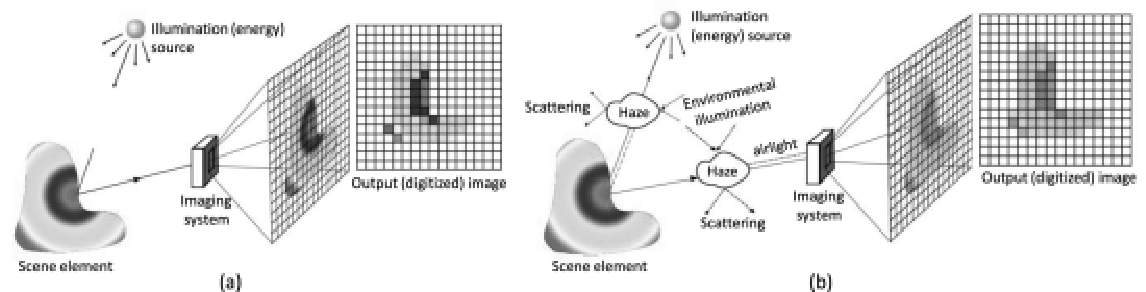
\includegraphics[width=0.8\textwidth]{figures/intro.png}
    \caption{Imaging Model}
\end{figure}

\end{itemize}

\end{frame}
%-----------------------------------------------------------------------------------
\begin{frame}[t]{Drak Channel Prior (DCP)}

\item{The dark channel prior is based on the statistics of haze-free outdoor image}
\item{Except sky region most of the local patches in the image have low intensity in atleast one color channel}
\item{In haze image intensity of these dark pixels change due to haze}
\item{These dark pixels provide estimate of the haze transmission.}
\begin{figure}[htbp!]
    \centering
    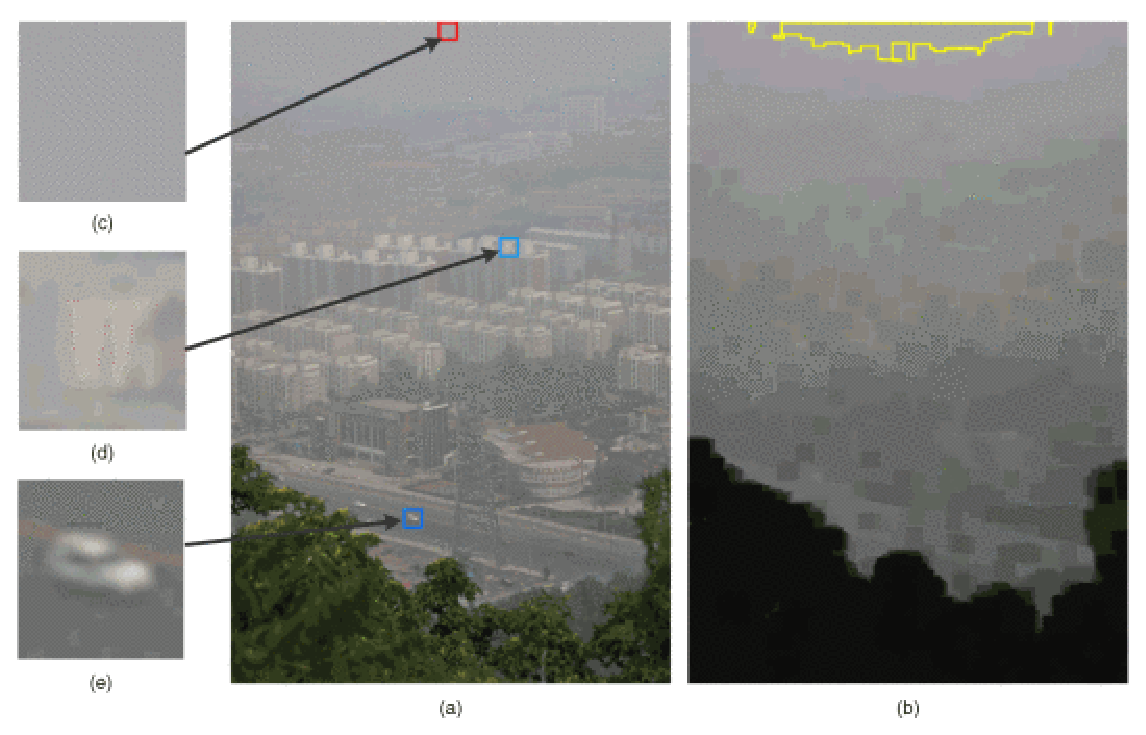
\includegraphics[width=0.5\textwidth]{figures/dcp.pdf}
    \caption{DCP and Atmospheric Light}
\end{figure}
\end{frame}

\begin{frame}[t]{Color Attenuation Prior (CAP)}
\item{Haze free patches have high saturation}
\item{Saturation decreases and brigthness increases due to Haze}
\item{Brightness decreases becauses of direct attenuation}
\begin{figure}[htbp!]
    \centering
    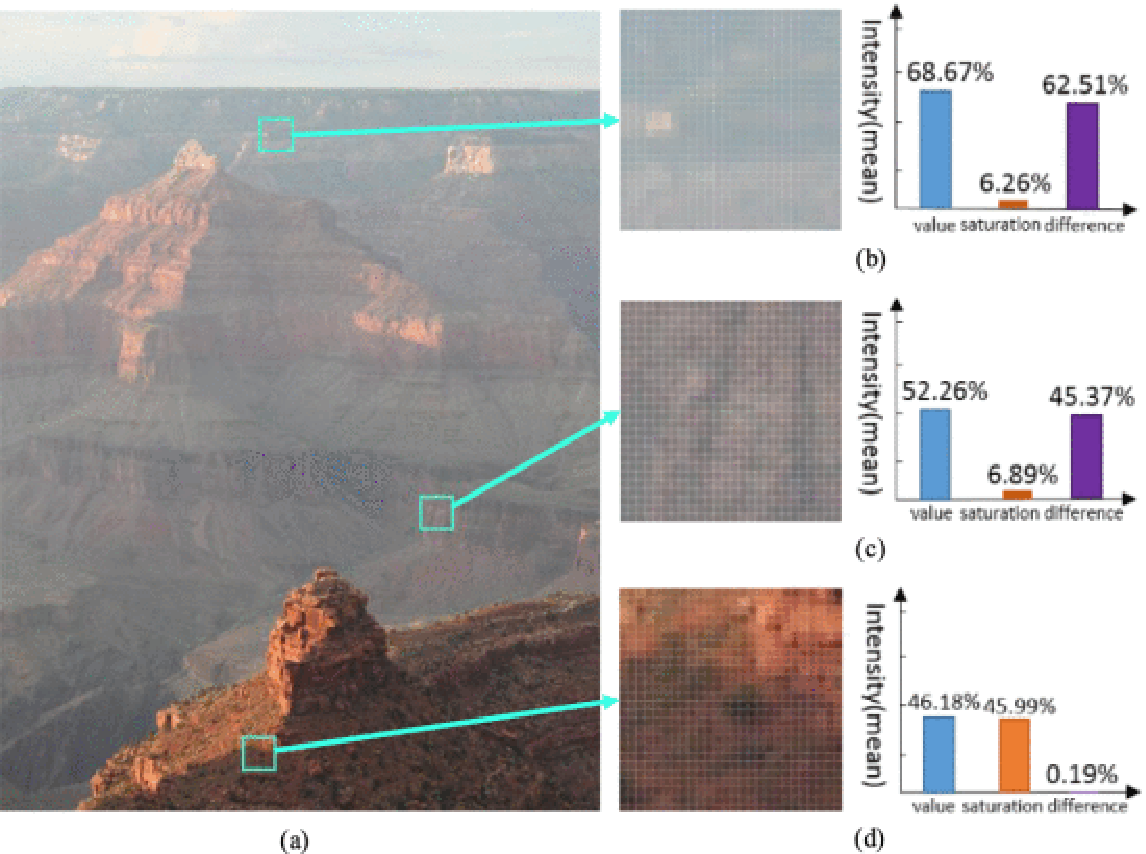
\includegraphics[width=0.5\textwidth]{figures/cap.pdf}
    \caption{CAP and Atmospheric Light}
\end{figure}

\end{frame}
\begin{frame}[t]{System Model}
\item{Atmospheric Scattering Model}
\begin{align} {{\mathbf{I}}}(x)=&{{\mathbf{J}}}(x)t(x)+{{\mathbf{A}}}(1-t(x)),
 \\ t(x)=&e^{-\beta d(x)} 
\end{align}

\item{I - hazy image}
\item{J - haze-free image}
\item{A - atmospheric light}
\item{t - medium transmission}
\item{$\beta$ - scattering coefficient of the atmosphere}
\item{d - depth of scene}

\end{frame}

\begin{frame}[t]{Transmission Map(DCP)}

\begin{figure}[htbp!]
 \begin{minipage}[b]{0.45\linewidth}
    \includegraphics[width=1.0\textwidth]{figures/mountain.png}
    \caption{Input Image with Haze}
\end{minipage}
    \begin{minipage}[b]{0.45\linewidth}
    \includegraphics[width=1.0\textwidth]{figures/t_mountain.png}
    \caption{Transmission Map}
	\end{minipage}   
\end{figure}


\end{frame}

\begin{frame}[t]{Depth Map extraction}

\begin{figure}[htbp!]
 \begin{minipage}[b]{0.45\linewidth}
    \includegraphics[width=1.0\textwidth]{figures/a.png}
    
\end{minipage}
\begin{minipage}[b]{0.45\linewidth}
    \includegraphics[width=1.0\textwidth]{figures/b.jpg}
   
\end{minipage}   
\end{figure}
\begin{figure}[htbp!]
 \begin{minipage}[b]{0.45\linewidth}
    \includegraphics[width=1.0\textwidth]{figures/c.png}
    
\end{minipage}
\begin{minipage}[b]{0.45\linewidth}
    \includegraphics[width=1.0\textwidth]{figures/d.png}
  
\end{minipage}   
\end{figure}


\end{frame}

\begin{frame}[t]{Capping of transmission}

\begin{figure}[htbp!]
 \begin{minipage}[b]{0.5\linewidth}
    \includegraphics[width=1.0\textwidth]{figures/dehazed_with_minmax.png}
    \caption{Transmission between 0.1 and 0.9}
\end{minipage}
    \begin{minipage}[b]{0.5\linewidth}
    \includegraphics[width=1.0\textwidth]{figures/dehazed_without_minmax.png}
\caption{Transmission uncapped}
	\end{minipage}   
\end{figure}


\end{frame}

\begin{frame}[t]{Simulation Results}

\begin{figure}[htbp!]
 \begin{minipage}[b]{0.45\linewidth}
    \includegraphics[width=1.0\textwidth]{figures/canon7.jpg}
    
\end{minipage}
    \begin{minipage}[b]{0.45\linewidth}
    \includegraphics[width=1.0\textwidth]{figures/mountain.png}

	\end{minipage}   
\end{figure}
\caption{Input Images with Haze}

\end{frame}



\end{frame}
\begin{frame}[t]{Simulation Results}

\begin{figure}[htbp!]
 \begin{minipage}[b]{0.45\linewidth}
    \includegraphics[width=1.0\textwidth]{figures/J_canon7.jpg}
    \caption{Dehazed using DCP}
\end{minipage}
    \begin{minipage}[b]{0.45\linewidth}
    \includegraphics[width=1.0\textwidth]{figures/8.png}
    \caption{Dehazed using CAP}
	\end{minipage}   
\end{figure}


\end{frame}


\begin{frame}[t]{Simulation Results}
\begin{figure}[htbp!]
 \begin{minipage}[b]{0.45\linewidth}
    \includegraphics[width=1.0\textwidth]{figures/J_mountain.png}
    \caption{Haze removal using DCP}
\end{minipage}
    \begin{minipage}[b]{0.45\linewidth}
    \includegraphics[width=1.0\textwidth]{figures/1.png}
    \caption{Haze removal using CAP}
	\end{minipage}   
\end{figure}



\end{frame}
%-------------------------------------------------------------------------------
\begin{frame}[t]{References}
\vspace{0.6cm}

\begin{thebibliography}{5}
\bibitem{1}
F. Fernandes and A. Ashikhmin and T. L. Marzetta, "Inter-Cell Interference in Noncooperative TDD Large Scale Antenna Systems",\textit{IEEE Journal on Selected Areas in Communications}, vol. IT-31, pp. 192-201, 2013.

\bibitem{2}
Thomas L. Marzetta, "Noncooperative Cellular Wireless with
Unlimited Numbers of Base Station Antennas.",\textit{IEEE transactions on Wireless Communications}  Vol. 9, no. 11, November 2010

\bibitem{3}
Jubin Jose, Alexei Ashikhmin, Thomas L. Marzetta and Sriram Vishwanath,"Pilot Contamination and Precoding in
Multi-Cell TDD Systems", \textit{
IEEE transactions on Wireless Communications}, Vol. 10, no. 8, August 2011

\end{thebibliography} 

\end{frame}

%--------------------------------------------------------------------------------
\begin{frame}[t]
\vspace{3cm}
\centering
\textbf{\Huge{Thank you}}
\end{frame}

%---------------------------------------------------------------------------------

\end{document}

